
\documentclass[landscape,final]{baposter}


\usepackage{times}
\usepackage{calc}
\usepackage{graphicx}
\usepackage{amsmath}
\usepackage{amssymb}
\usepackage{relsize}
\usepackage{multirow}
\usepackage{bm}
\usepackage{epstopdf}
\usepackage{setspace}
\usepackage{graphicx}
\usepackage{multicol}
\usetikzlibrary{arrows}
\usepackage{mathtools,bm}
\usepackage{vwcol}
\usepackage{qrcode}  % Add this line


\usepackage{pgfbaselayers}
\pgfdeclarelayer{background}
\pgfdeclarelayer{foreground}
\pgfsetlayers{background,main,foreground}

\usepackage{helvet}
%\usepackage{bookman}
\usepackage{palatino}
\newcommand{\cK}{\mathcal{K}}




\newcommand{\captionfont}{\footnotesize}

\selectcolormodel{cmyk}

%\graphicspath{{images/}}

%\graphicspath{{figures/}}



%%%%%%%%%%%%%%%%%%%%%%%%%%%%%%%%%%%%%%%%%%%%%%%%%%%%%%%%%%%%%%%%%%%%%%%%%%%%%%%%
%%%% Some math symbols used in the text
%%%%%%%%%%%%%%%%%%%%%%%%%%%%%%%%%%%%%%%%%%%%%%%%%%%%%%%%%%%%%%%%%%%%%%%%%%%%%%%%
% Format 
\newcommand{\Matrix}[1]{\begin{bmatrix} #1 \end{bmatrix}}
\newcommand{\Vector}[1]{\Matrix{#1}}
\newcommand*{\SET}[1]  {\ensuremath{\mathcal{#1}}}
\newcommand*{\MAT}[1]  {\ensuremath{\mathbf{#1}}}
\newcommand*{\VEC}[1]  {\ensuremath{\bm{#1}}}
\newcommand*{\CONST}[1]{\ensuremath{\mathit{#1}}}
\newcommand*{\norm}[1]{\mathopen\| #1 \mathclose\|}% use instead of $\|x\|$
\newcommand*{\abs}[1]{\mathopen| #1 \mathclose|}% use instead of $\|x\|$
\newcommand*{\absLR}[1]{\left| #1 \right|}% use instead of $\|x\|$

\def\norm#1{\mathopen\| #1 \mathclose\|}% use instead of $\|x\|$
\newcommand{\normLR}[1]{\left\| #1 \right\|}% use instead of $\|x\|$

\newcommand{\pd}{\partial}
\newcommand{\fns}{\footnotesize}
\newcommand{\ns}{\normalsize}
\newcommand{\scs}{\scriptsize}
\newcommand{\dd}{{\rm d}}
\newcommand{\e}{{\rm e}}
\newcommand{\Z}{{\mathbb Z}}
\newcommand{\mc}{\mathcal}
\newcommand{\ep}{\epsilon}
\renewcommand{\d}{{\rm d}}

%%%%%%%%%%%%%%%%%%%%%%%%%%%%%%%%%%%%%%%%%%%%%%%%%%%%%%%%%%%%%%%%%%%%%%%%%%%%%%%%
% Multicol Settings
%%%%%%%%%%%%%%%%%%%%%%%%%%%%%%%%%%%%%%%%%%%%%%%%%%%%%%%%%%%%%%%%%%%%%%%%%%%%%%%%
\setlength{\columnsep}{0.7em}
\setlength{\columnseprule}{0mm}


%%%%%%%%%%%%%%%%%%%%%%%%%%%%%%%%%%%%%%%%%%%%%%%%%%%%%%%%%%%%%%%%%%%%%%%%%%%%%%%%
% Save space in lists. Use this after the opening of the list
%%%%%%%%%%%%%%%%%%%%%%%%%%%%%%%%%%%%%%%%%%%%%%%%%%%%%%%%%%%%%%%%%%%%%%%%%%%%%%%%
\newcommand{\compresslist}{%
\setlength{\itemsep}{1pt}%
\setlength{\parskip}{0pt}%
\setlength{\parsep}{0pt}%
}

\usepackage{enumitem}
\setlist[itemize,1]{leftmargin=\dimexpr 26pt-0.22in}

\DeclareMathSizes{10}{9}{7}{6}
\DeclareSymbolFont{extraup}{U}{zavm}{m}{n}
\DeclareMathSymbol{\vardiamond}{\mathalpha}{extraup}{87}




%%%%%%%%%%%%%%%%%%%%%%%%%%%%%%%%%%%%%%%%%%%%%%%%%%%%%%%%%%%%%%%%%%%%%%%%%%%%%%
%%% Begin of Document
%%%%%%%%%%%%%%%%%%%%%%%%%%%%%%%%%%%%%%%%%%%%%%%%%%%%%%%%%%%%%%%%%%%%%%%%%%%%%%

\begin{document}

%%%%%%%%%%%%%%%%%%%%%%%%%%%%%%%%%%%%%%%%%%%%%%%%%%%%%%%%%%%%%%%%%%%%%%%%%%%%%%
%%% Here starts the poster
%%%---------------------------------------------------------------------------
%%% Format it to your taste with the options
%%%%%%%%%%%%%%%%%%%%%%%%%%%%%%%%%%%%%%%%%%%%%%%%%%%%%%%%%%%%%%%%%%%%%%%%%%%%%%
\typeout{Poster Starts}
\background{
  \begin{tikzpicture}[remember picture,overlay]%
    \draw (current page.north west)+(-2em,-0em) node[anchor=north west] {\hspace{-2em}\includegraphics[height=1.1\textheight]{silhouettes_background}};
  \end{tikzpicture}%
}
\definecolor{silver}{cmyk}{0,0,0,0.1}
\definecolor{yellow}{cmyk}{0,0,0.9,0.0}
\definecolor{reddishyellow}{cmyk}{0,0.22,1.0,0.0}
\definecolor{black}{cmyk}{0,0,0.0,1.0}
\definecolor{darkYellow}{cmyk}{0,0,1.0,0.5}
\definecolor{darkSilver}{cmyk}{0,0,0,0.1}
\definecolor{red}{cmyk}{0,1,1,0.07}
\definecolor{white}{cmyk}{0,0,0,0}

\definecolor{lightyellow}{cmyk}{0,0,0.3,0.0}
\definecolor{lighteryellow}{cmyk}{0,0,0.15,0.0}
\definecolor{lighteryellow}{cmyk}{0,0,0.15,0.0}
\definecolor{lightestyellow}{cmyk}{0,0,0.05,0.0}
\definecolor{lightestblue}{cmyk}{0.15,0.06,0,0}
\definecolor{lightblue}{cmyk}{0.21,0.12,0,0.13}
\definecolor{slateblue}{cmyk}{1,0.5,0,0}
\definecolor{lightpink}{rgb}{0.5, 0.6, 0.7}

\begin{poster}{
  % Show grid to help with alignment
  grid=no,
  columns=3,
  % Column spacing
  colspacing=1em,
  % Color style
%  bgColorOne=lighteryellow,
%  bgColorTwo=lighteryellow,
bgColorOne=silver,
  bgColorTwo=lightestblue,
  borderColor=black,
  headerColorOne=black,
%  headerColorOne=reddishyellow,
  headerColorTwo=reddishyellow,
    headerFontColor=white,
%  headerFontColor=black,
%  boxColorOne=lightestblue,
%  boxColorTwo=lightestblue,
  boxColorOne=white,
  boxColorTwo=white,
  % Format of textbox
  textborder=roundedleft,
  % Format of text header
  eyecatcher=yes,
  headerborder=closed,
  headerheight=0.10\textheight,
  headershape=rectangle,
  headershade=plain,
  headerfont=\Large\textsf, %Sans Serif
  boxshade=plain,
%  background=shade-tb,
  background=plain,
  linewidth=2pt
  }
  % Eye Catcher
  {{\begin{minipage}{5.3em}
  			\includegraphics[height=6em]{images/ComputerScience_bw_center_transparent.png}
  			%%%%%%%%%%%%%%%%%%%%%%%%%%%%%%%%%%%%%%%%%%%%%%%%%%%%%%%%%%%%%%%%%%%%%%%%%%%%%%%%%%%%%%%%%%
  \end{minipage}}} % No eye catcher for this poster. If an eye catcher is present, the title is centered between eye-catcher and logo.
  % Title
 {% \sc %Sans Serif
  \bf %Serif
   \huge Adaptive Mesh Refinement for Obstacle Problems
   }
    % Authors
  {\sc %Sans Serif
    % Serif
  \begin{center} {
  \large Stefano Fochesatto$^{1}$ and Ed Bueler$^{2}$\\ \normalsize 1:\,University of Colorado Boulder; 2:\,University of Alaska Fairbanks
  }  
  \end{center}
  }
  % University logo 
 {{\begin{minipage}{7.5em}
  \centering
  \includegraphics[height=7.5em]{images/top_part.png}\\[-2.75mm]
  \includegraphics[width=7.5em]{images/caption.png}[-2mm]
  \end{minipage}}}
  % Width of left inset image
     \newlength{\leftimgwidth}
     \setlength{\leftimgwidth}{0.78em+8.0em}

%%%%%%%%%%%%%%%%%%%%%%%%%%%%%%%%%%%%%%%%%%%%%%%%%%%%%%%%%%%%%%%%%%%%%%%%%%%%%%
%%% Now define the boxes that make up the poster
%%%---------------------------------------------------------------------------
%%% Each box has a name and can be placed absolutely or relatively.
%%% The only inconvenience is that you can only specify a relative position 
%%% towards an already declared box. So if you have a box attached to the 
%%% bottom, one to the top and a third one which should be in between, you 
%%% have to specify the top and bottom boxes before you specify the middle 
%%% box.
%%%%%%%%%%%%%%%%%%%%%%%%%%%%%%%%%%%%%%%%%%%%%%%%%%%%%%%%%%%%%%%%%%%%%%%%%%%%%%
    %
    % A coloured circle useful as a bullet with an adjustably strong filling
    \newcommand{\colouredcircle}[1]{%
      \tikz{\useasboundingbox (-0.2em,-0.32em) rectangle(0.2em,0.32em); \draw[draw=black,fill=baposterBGone!80!black!#1!white,line width=0.03em] (0,0) circle(0.18em);}}
%%%%%%%%%%%%%%%%%%%%%%%%%%%%%%%%%%%%%%%%%%%%%%%%%%%%%%%%%%%%%%%%%%%%%%%%%%%%%%
  \headerbox{\ns \textbf{Introduction:} Classical Obstacle Problem}{name=summary,column=0,row=0}{
%%%%%%%%%%%%%%%%%%%%%%%%%%%%%%%%%%%%%%%%%%%%%%%%%%%%%%%%%%%%%%%%%%%%%%%%%%%%%%
 \begin{spacing}{0.8}  {\footnotesize
% \raggedright
\begin{center}  
  \includegraphics[width=0.9\textwidth]{../../../paper/static/obstacle.png}
\end{center}
\begin{center}
Solve for the displacement of an elastic membrane $u(x, y)$ over a region $\Omega$ which minimizes elastic potential energy, subject to a distributed load $f(x, y)$,  $u|_{\partial \Omega} =  g$ and $u \geq \psi$ \cite{KinderlehrerStampacchia1980}. 
\end{center}

\noindent\rule{\textwidth}{0.4pt}

\vspace{1mm}

\begin{minipage}[t]{0.40\textwidth}
\begin{itemize}
\setlength\itemsep{0pt}
\item \textbf{Energy Minimization:} \\
Let $K_\psi = \{v \in H^1_{g}(\Omega)| v \geq \psi\}$,
\begin{align*}
\underset{u \in K_\psi}{\text{minimize: }} I(u) = \int_\Omega \frac{1}{2} \abs{\nabla u}^2 - fu
\end{align*}
\end{itemize}
\end{minipage}
\hspace{1mm}
\vrule
\hspace{1mm}
\begin{minipage}[t]{0.50\textwidth}
\begin{itemize}
\setlength\itemsep{0pt}
\item \textbf{Complementarity Problem (CP):} \\
For $u \in C(\overline{\Omega}) \cap C^2(\Omega)$, the following hold over $\Omega$ a.e.:
\begin{align*}
-\nabla^2 u - f &\geq 0 \\
u - \psi &\geq 0 \\
(-\nabla^2u - f)(u - \psi) &= 0
\end{align*}
\end{itemize}
\end{minipage}
\vspace{1mm}

\noindent\rule{\textwidth}{0.4pt}
\vspace{1mm}


% Figure and bullets side by side
\begin{minipage}[c]{0.38\textwidth}
\centering
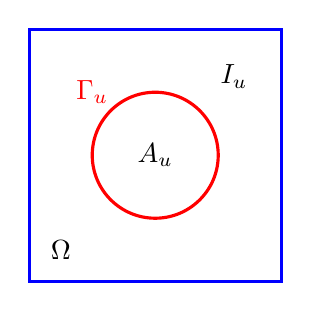
\begin{tikzpicture}[scale=0.8]
% Draw the square with blue line and label
\draw[line width=0.4mm, blue] (0,0) rectangle (4,4);
\node at (0.5,0.5) {$\Omega$};
% Draw the circle with red line
\draw[line width=0.4mm, red] (2,2) circle (1cm);
\node at (2,2) {{$A_u$}};
\node at (1,3) {\textcolor{red}{$\Gamma_u$}};
% Label the region between the circle and the square
\node at (3.25,3.25) {$I_u$};
\end{tikzpicture}
\end{minipage}
\hfill
\begin{minipage}[c]{0.58\textwidth}
\begin{itemize}
\setlength\itemsep{0pt}
\item The solution $u$ defines:
\begin{itemize}
\item Active Set $A_u = \{u = \psi\}$ (Data)
\item Inactive Set $I_u = \{u > \psi\}$ (PDE region)
\item Free Boundary $\Gamma_u = \partial I_u \cap \Omega$
\end{itemize}
\item On the free boundary $\Gamma_u$:
\begin{itemize}
\item $u = \psi$
\item $u' = \psi'$
\end{itemize}
\end{itemize}
\end{minipage}
\vspace{5mm}
} \end{spacing} 
\ \\
\vspace{-6mm}
 }



%%%%%%%%%%%%%%%%%%%%%%%%%%%%%%%%%%%%%%%%%%%%%%%%%%%%%%%%%%%%%%%%%%%%%%%%%%%%%%
  \headerbox{{\ns \small \textbf{Motivations and Approach:} \footnotesize{Free Boundary Adaptive Mesh Refinement (AMR)}}}{name=model,column=0,below=summary}{
%%%%%%%%%%%%%%%%%%%%%%%%%%%%%%%%%%%%%%%%%%%%%%%%%%%%%%%%%%%%%%%%%%%%%%%%%%%%%%
  
\footnotesize

\begin{itemize}
\item AMR for PDEs
\begin{itemize}
  \item Refine mesh in regions of high solution error, coarsen in regions of low error, to efficiently capture solution features.
\end{itemize}
\item AMR for Variational Inequalities (VIs)
\begin{itemize}
  \item Often the simulation goal is localization of the free boundary $\Gamma_u$.
  \item Resolution in a stabilized $A_u$ is unnecessary since $u = \psi$. 
  \item Standard PDE error estimators cannot be applied to all of $\Omega$ in a VI problem.
  \item Poorly localized $\Gamma_u$ can produce dominating error in $I_{u_h}$.
\end{itemize}

\item Our Approach: Free Boundary Aware AMR
\begin{itemize}
  \item Use Grid Sequencing and refine near $\Gamma_{u_h}$, the discrete free boundary.
  \item Use PDE error indicators to refine in $I_{u_h}$, the discrete inactive set.
\end{itemize}
\end{itemize}
\vspace{1mm}
}


%%%%%%%%%%%%%%%%%%%%%%%%%%%%%%%%%%%%%%%%%%%%%%%%%%%%%%%%%%%%%%%%%%%%%%%%%%%%%%
  \headerbox{{\ns \textbf{Methods:} VCD and UDO Strategies}}{name=existence,column=1,row=0}{
%%%%%%%%%%%%%%%%%%%%%%%%%%%%%%%%%%%%%%%%%%%%%%%%%%%%%%%%%%%%%%%%%%%%%%%%%%%%%%
\footnotesize
\begin{itemize}
\item \textbf{Variable Coefficient Diffusion (VCD)}
\end{itemize}
\vspace{-5mm}
\begin{center}
\resizebox{\textwidth}{!}{%
  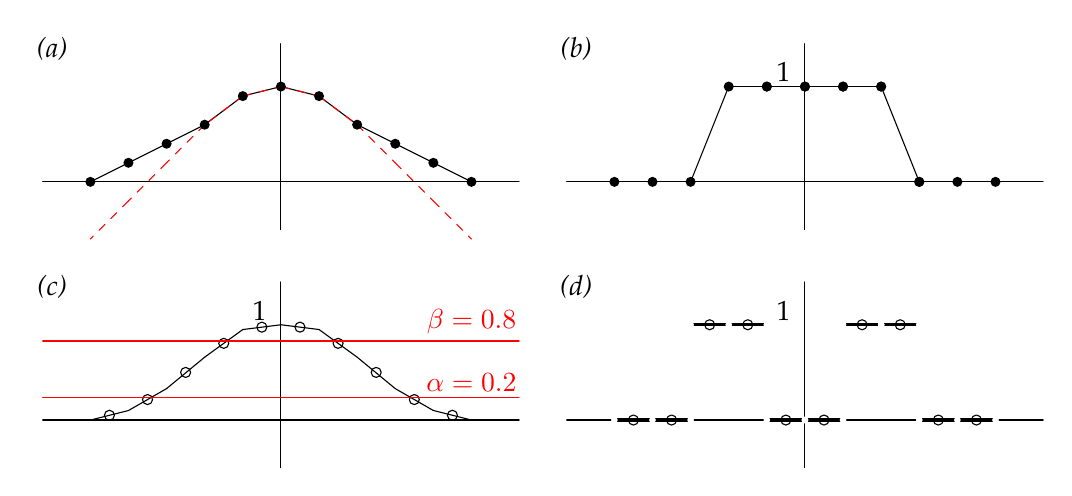
\begin{tikzpicture}[line cap=round,line join=round,>=triangle 45,scale=1.21]

%%%%%% (a) %%%%%
    \draw (0.4,0.9) -- (0.8,0.6);
    \draw (0.8,0.6) -- (1.2,0.4);
    \draw (1.2,0.4) -- (1.6,0.2);
    \draw (-0.4,0.9) -- (-0.8,0.6);
    \draw (-0.8,0.6) -- (-1.2,0.4);
    \draw (-1.2,0.4) -- (-1.6,0.2);
    \draw (-1.6,0.2) -- (-2,0);
    \draw (1.6,0.2) -- (2,0);
    \draw (-0.4,0.9) -- (0,1);
    \draw (0,1) -- (0.4,0.9);

    % New red curve aligning with black nodes
    \draw[red,dashed] (1.6,-.2) -- (2,-.6);
    \draw[red,dashed] (1.2,0.2) -- (1.6,-.2);
    \draw[red,dashed] (0.8,0.6) -- (1.2,0.2);
    \draw[red,dashed] (0.4,0.9) -- (0.8,0.6);
    \draw[red,dashed] (0,1) -- (0.4,0.9);
    \draw[red,dashed] (-0.4,0.9) -- (0,1);
    \draw[red,dashed] (-0.4,0.9) -- (-0.8,0.6);
    \draw[red,dashed] (-0.8,0.6) -- (-1.2,.2);
    \draw[red,dashed] (-1.2, .2) -- (-1.6,-.2);
    \draw[red,dashed] (-1.6,-.2) -- (-2,-.6);

    \begin{scriptsize}
      \fill [color=black] (-0.4,0.9) circle (1.5pt);
      \fill [color=black] (0.4,0.9) circle (1.5pt);
      \fill [color=black] (0.8,0.6) circle (1.5pt);
      \fill [color=black] (1.2,0.4) circle (1.5pt);
      \fill [color=black] (1.6,0.2) circle (1.5pt);
      \fill [color=black] (-0.8,0.6) circle (1.5pt);
      \fill [color=black] (-1.2,0.4) circle (1.5pt);
      \fill [color=black] (-1.6,0.2) circle (1.5pt);
      \fill [color=black] (-2,0) circle (1.5pt);
      \fill [color=black] (2,0) circle (1.5pt);
      \fill [color=black] (0,1) circle (1.5pt);
    \end{scriptsize}

    % Add Axes
    \draw[-] (-2.5,0) -- (2.5,0); % x-axis
    \draw[-] (0,-0.5) -- (0,1.45); % y-axis

    \node at (-2.4,1.4) {\emph{(a)}};


%%%%%% (b) %%%%%
\begin{scope}[shift={(5.5,0.0)}]
    \draw (1.6,0) -- (2,0);
    \draw (1.2,0) -- (1.6,0);
    \draw (0.8,1) -- (1.2,0);
    \draw (0.4,1) -- (0.8,1);
    \draw (0,1) -- (0.4,1);
    \draw (-0.4,1) -- (0,1);
    \draw (-0.4,1) -- (-0.8,1);
    \draw (-0.8,1) -- (-1.2,0);
    \draw (-1.2,0) -- (-1.6,0);
    \draw (-1.6,0) -- (-2,0);

    % Add black vertices
    \begin{scriptsize}
      \fill [color=black] (1.6,0) circle (1.5pt);
      \fill [color=black] (2,0) circle (1.5pt);
      \fill [color=black] (1.2,0) circle (1.5pt);
      \fill [color=black] (0.8,1) circle (1.5pt);
      \fill [color=black] (1.2,0) circle (1.5pt);
      \fill [color=black] (0.4,1) circle (1.5pt);
      \fill [color=black] (0.8,1) circle (1.5pt);
      \fill [color=black] (0,1) circle (1.5pt);
      \fill [color=black] (0.4,1) circle (1.5pt);
      \fill [color=black] (-0.4,1) circle (1.5pt);
      \fill [color=black] (0,1) circle (1.5pt);
      \fill [color=black] (-0.4,1) circle (1.5pt);
      \fill [color=black] (-0.8,1) circle (1.5pt);
      \fill [color=black] (-1.2,0) circle (1.5pt);
      \fill [color=black] (-1.6,0) circle (1.5pt);
      \fill [color=black] (-2,0) circle (1.5pt);
    \end{scriptsize}
    
    % Add Axes
    \draw[-] (-2.5,0) -- (2.5,0); % x-axis
    \draw[-] (0,-0.5) -- (0,1.45); % y-axis

    % Label y=1
    \node at (-0.05,1.15) [left] {1};

    \node at (-2.4,1.4) {\emph{(b)}};
\end{scope}


%%%%%% (c) %%%%%
\begin{scope}[shift={(0.0,-2.5)}]
    % Draw the smoothed curve
    \draw (1.6, 0.1) -- (2,0);      
    \draw (1.2, 0.33) -- (1.6, 0.1);
    \draw (0.8, 0.66) -- (1.2, 0.33);
    \draw (0.4, 0.95) -- (0.8, 0.66);
    \draw (0,1) -- (0.4, 0.95);
    \draw (-0.4, 0.95) -- (0,1);
    \draw (-0.4, 0.95) -- (-0.8, 0.66);
    \draw (-0.8, 0.66) -- (-1.2, 0.33);
    \draw (-1.2, 0.33) -- (-1.6, 0.1);
    \draw (-1.6, 0.1) -- (-2,0);

    % Add black circles at element centers
    \begin{scriptsize}
      \draw [color=black] (1.8, 0.05) circle (1.5pt);
      \draw [color=black] (1.4, 0.215) circle (1.5pt);
      \draw [color=black] (1.0, 0.5) circle (1.5pt);
      \draw [color=black] (0.6, 0.805) circle (1.5pt);
      \draw [color=black] (0.2, 0.975) circle (1.5pt);
      \draw [color=black] (-0.2, 0.975) circle (1.5pt);
      \draw [color=black] (-0.6, 0.805) circle (1.5pt);
      \draw [color=black] (-1.0, 0.5) circle (1.5pt);
      \draw [color=black] (-1.4, 0.215) circle (1.5pt);
      \draw [color=black] (-1.8, 0.05) circle (1.5pt);
    \end{scriptsize}

    % Add Axes
    \draw[-] (-2.5,0) -- (2.5,0); % x-axis
    \draw[-] (0,-0.5) -- (0,1.45); % y-axis

    % Label y=1
    \node at (-0.05,1.15) [left] {1};

    % Add red horizontal lines; pretend heights are 0.8 and 0.2
    \draw[red] (-2.5, 0.83) -- (2.5, 0.83);
    \draw[red] (-2.5, 0.24) -- (2.5, 0.24);
    % Label the heights of the red lines
    \node[red] at (2, 0.8) [above] {$\beta=0.8$};
    \node[red] at (2, 0.2) [above] {$\alpha=0.2$};

    \node at (-2.4,1.4) {\emph{(c)}};
\end{scope}


%%%%%% (d) %%%%%
\begin{scope}[shift={(5.5,-2.5)}]

    \draw[very thick] (1.6,0) -- (2,0);      
    \draw[very thick] (1.2,0) -- (1.6,0);
    \draw[very thick] (0.8,1) -- (1.2,1);
    \draw[very thick] (0.4,1) -- (0.8,1);
    \draw[very thick] (0,0) -- (0.4,0);
    \draw[very thick] (-0.4,0) -- (0,0);
    \draw[very thick] (-0.4,1) -- (-0.8,1);
    \draw[very thick] (-0.8,1) -- (-1.2,1);
    \draw[very thick] (-1.2,0) -- (-1.6,0);
    \draw[very thick] (-1.6,0) -- (-2,0);

    % Add Axes
    \draw[-] (-2.5,0) -- (2.5,0); % x-axis
    \draw[-] (0,-0.5) -- (0,1.45); % y-axis

    % Label y=1
    \node at (-0.05,1.15) [left] {1};

    % Add Nodes in white to separate elements
    \begin{scriptsize}
    \fill [color=white] (1.6,0) circle (1.0pt);
    \fill [color=white] (2,0) circle (1.0pt);      
    \fill [color=white] (1.2,0) circle (1.0pt);
    \fill [color=white] (0.8,1) circle (1.0pt);
    \fill [color=white] (1.2,1) circle (1.0pt);
    \fill [color=white] (0.4,1) circle (1.0pt);
    \fill [color=white] (0.8,1) circle (1.0pt);
    \fill [color=white] (0,0) circle (1.0pt);
    \fill [color=white] (0.4,0) circle (1.0pt);
    \fill [color=white] (-0.4,0) circle (1.0pt);
    \fill [color=white] (0,0) circle (1.0pt);
    \fill [color=white] (-0.4,1) circle (1.0pt);
    \fill [color=white] (-0.8,1) circle (1.0pt);
    \fill [color=white] (-1.2,1) circle (1.0pt);
    \fill [color=white] (-1.2,0) circle (1.0pt);
    \fill [color=white] (-1.6,0) circle (1.0pt);
    \fill [color=white] (-2,0) circle (1.0pt);
    \end{scriptsize}

    % Add black circles at element centers
    \begin{scriptsize}
      \draw [color=black] (1.8, 0.0) circle (1.5pt);
      \draw [color=black] (1.4, 0.0) circle (1.5pt);
      \draw [color=black] (1.0, 1.0) circle (1.5pt);
      \draw [color=black] (0.6, 1.0) circle (1.5pt);
      \draw [color=black] (0.2, 0.0) circle (1.5pt);
      \draw [color=black] (-0.2, 0.0) circle (1.5pt);
      \draw [color=black] (-0.6, 1.0) circle (1.5pt);
      \draw [color=black] (-1.0, 1.0) circle (1.5pt);
      \draw [color=black] (-1.4, 0.0) circle (1.5pt);
      \draw [color=black] (-1.8, 0.0) circle (1.5pt);
    \end{scriptsize}

    \node at (-2.4,1.4) {\emph{(d)}};
\end{scope}

\end{tikzpicture}
}% end resizebox
\end{center}
\begin{center}
\textit{(a) $\psi$ in red, $u_h$ in black. (b) Nodal $A_{u_h}$ indicator. (c) Smoothed $A_{u_h}$ indicator with thresholds $\alpha$ and $\beta$. (d) Final element indicator for refinement.}
\end{center}

\begin{itemize}
  \item \textbf{Unstructured Dilation Operator (UDO)}
\end{itemize}
\vspace{-7mm}
\begin{center}
\begin{tabular}{ccc}
\begin{minipage}{0.3\textwidth}
\centering
\includegraphics[width=\textwidth]{Figures/UDOIllustration/000.png}
\emph{(a)}
\end{minipage} &
\begin{minipage}{0.3\textwidth}
\centering
\includegraphics[width=\textwidth]{Figures/UDOIllustration/002.png}
\emph{(b)}
\end{minipage} &
\begin{minipage}{0.3\textwidth}
\centering
\includegraphics[width=\textwidth]{Figures/UDOIllustration/003.png}
\emph{(c)}
\end{minipage}
\end{tabular}
\end{center}

\begin{center}
\textit{(a) $u_h$ with $\Gamma_{u_h}$ in green. (b) Computed border elements indicator. (c) Final one-neighbor refinement indicator.}
\end{center}
	
}


\headerbox{\ns \textbf{Results:} Metric for $\Gamma_{u_h}$ Convergence}{name=stability1,column=1,span=1,below=existence}{
  \footnotesize

  \begin{minipage}[t]{0.48\textwidth}
  \begin{itemize}
  \setlength\itemsep{0pt}
  \item \textbf{Preferred Approximation:}
   $$\tilde{u}_h(x) = \begin{cases} \psi(x) & x \in A_u^h \\ u_h(x) & \text{otherwise} \end{cases}$$
  \end{itemize}
  \end{minipage}
  \hspace{1mm}
  \vrule
  \hspace{1mm}
  \begin{minipage}[t]{0.48\textwidth}
  \begin{itemize}
  \setlength\itemsep{0pt}
  \item \textbf{Jaccard Distance \cite{LevandowskyWinter1971}:} \\ Let $S,T \subset \Omega$ be measurable sets, then
  $$d(S,T) = 1 - \frac{|S \cap T|}{|S \cup T|}$$
  where $|\cdot|$ is Lebesgue measure.
  \end{itemize}
  \end{minipage}
  \vspace{1mm}

  \noindent\rule{\textwidth}{0.4pt}

  \vspace{-2mm}
  \begin{itemize}
    \item  \textbf{Reference Sphere Obstacle Problem (Chapter 13, \cite{Bueler2021}).}
  \end{itemize}
  \begin{center}
  \vspace{-5mm}
    
    \vspace{0.5em}
    \resizebox{\textwidth}{!}{%
    \begin{tabular}{cc}
      \includegraphics[width=0.48\textwidth]{../../../paper/genfigs/convball_VCD+BR.png} &
      \includegraphics[width=0.48\textwidth]{../../../paper/genfigs/jaccball.png}
    \end{tabular}
    }% end resizebox
  \end{center}
}




 \headerbox{\ns \textbf{Gallery:} Benchmark Problems }{name=conclusions1,column=2,row=0}{
  \begin{center}
    \textit{\footnotesize{Meshes generated by our methods for several benchmark problems. \\ Mesh in red, $A_{u_h}$ in black, $I_{u_h}$ in grey.}}
  \end{center}

  \vspace{-6mm}

  \begin{center}
  \resizebox{.95\textwidth}{!}{%
  \begin{tabular}{cc}
  \includegraphics[width=0.48\textwidth]{../../../paper/static/spiralmesh.png} &
  \includegraphics[width=0.48\textwidth]{../../../paper/static/lshaped.png} \\
  {\footnotesize Spiral \cite{GraeserKornhuber2009}} & {\footnotesize L-shaped} \\[1 mm]
  \includegraphics[width=0.48\textwidth]{../../../paper/static/blistersmesh.png} &
  \includegraphics[width=0.48\textwidth]{../../../paper/static/blisterszoomed.png} \\
  {\footnotesize Blisters} & {\footnotesize Blisters (zoomed)}
  \end{tabular}
  }% end resizebox
  \end{center}

 }

 %%%%%%%%%%%%%%%%%%%%%%%%%%%%%%%%%%%%%%%%%%%%%%%%%%%%%%%%%%%%%%%%%%%%%%%%%%%%%%
  \headerbox{\ns\textbf{Application:} Predicting Glaciated Land Areas}{name=conclusions2, column=2,below=conclusions1}{
  \footnotesize
  \begin{itemize}
    \item \textbf{Model \cite{Bueler2016}:} Shallow Ice Approximation (SIA) 
    $$
    \int_\Omega \Gamma |\nabla u + \mathbf{\beta}(u)|^2 (\nabla u + \mathbf{\beta}(u)) \cdot \nabla (v-u) - \tilde a(u) (v-u)\,dx \ge 0
    $$
  \end{itemize}

  \vspace{2mm}

  \begin{minipage}[t]{0.48\textwidth}
    \begin{itemize}
      \item \textbf{Physical ice thickness}: $H = u^{3/8}$
      \item \textbf{Ice surface elevation}: $s = u^{3/8} + b$
      \item \textbf{Bedrock elevation}: $b(x,y)$
      \item \textbf{Surface mass-balance}: $a(x,y,s)$
    \end{itemize}
  \end{minipage}
  \hfill
  \begin{minipage}[t]{0.48\textwidth}
    \begin{itemize}
      \item \textbf{Ice softness}: $\Gamma > 0$
      \item \textbf{Tilt term}: $\mathbf{\beta}(u)=\frac{8}{3} u^{5/8} \nabla b$
      \item $\tilde a(u)=a(x,y,s)$
      \item $u \in \cK = \{u \in W^{1,4}(\Omega)\,:\,u\ge 0 \text{ and } u|_{\partial\Omega}=0\}$
    \end{itemize}
  \end{minipage}

  \vspace{-3mm}

  \begin{center}
  \resizebox{.90\textwidth}{!}{%
  \begin{tabular}{cc}
    \begin{minipage}{0.48\textwidth}
      \centering
      \includegraphics[width=\textwidth]{../../../paper/genfigs/drmax.png}
      \vspace{2mm}
      \textit{Maximum radial error of the glacier margin.}
    \end{minipage} &
    \begin{minipage}{0.48\textwidth}
      \centering
      \includegraphics[width=\textwidth]{../../../paper/genfigs/herrinf.png}
      \vspace{2mm}
      \textit{Max error in the ice thickness $H$.}
    \end{minipage}
  \end{tabular}
  }% end resizebox
  \end{center}
}
 
%%%%%%%%%%%%%%%%%%%%%%%%%%%%%%%%%%%%%%%%%%%%%%%%%%%%%%%%%%%%%%%%%%%%%%%%%%%%%%

\end{poster}

\bibliographystyle{plain}
\bibliography{poster}

\end{document}